\chapter{Trash (in) Art}

\epigraph{One day, in a rubbish heap, I found an old bicycle seat lying beside a rusted handlebar, and my mind instantly linked them together. I assembled these two objects, which everyone then recognized as a bull’s head. The metamorphosis was accomplished, and I wish another metamorphosis would occur in the reverse sense. If my bull’s head were thrown in a junk heap, perhaps one day some boy would say, \quotes{Here’s something that would make a good handlebar for my bicycle!}}{\hfill ---Pablo Picasso, \textit{Trashformations}}

How and why does trash draw attention of artists(, and also mine)? In this chapter how artist approached to the trash and their techniques are discussed in the context of art. (Historical development, methodologies, tactics, motivations\ldots) Focused on visual (plastic) arts(, because there is also a music genre called as trash music?). How does it turn to medium?

% TODO List motivations of artists and their ideas about junk. Because it reveals the different dimensions of this topic.

%%%
%%%
%%%
\section{Root in the Art History}
In this chapter root of using ---(non-art)--- objects in the artworks is examined. In other words using objects in artworks beyond their intended purpose or intended meaning and function. Developing artworks not only painting but also using paper and other stuff by pasting them together. (Foundations of trash in art.) Using object apart from their proposed meaning is not a new thing[ref required, using jewelry by African tribes], through the ages people used objects and tools for different purposes. However it is not discussed in the context of (western)art and not accepted method for art making. Therefore who and which work introduces this concept and how it is developed and evolved in time. (of course it is a brief overview by some remarkable pieces.)

% TODO paraphrase
\quotes{The use of trash as a fine art medium dates back at least to the work of early-20th-century artists such as Fortunato Depero and Kurt Schwitters. Use of found materials, including garbage, has been associated with assemblage art since the 1950s and has been practiced by other well-known artists, including graphic artist Christian Boltanski, sculptor Louise Bourgeois, and photographer Andres Serrano. Art made from garbage has since become much more common in fine arts venues such as museums, galleries, and high-profile installations, including H. A. Schuldt’s famous “Trash People,” which has traveled around the world since 1996}  \cite{tauxe2012encyclopedia}.

%%
%%
\subsection{Collage}
Collage originates from the French \textit{coller} is an artistic technique of applying manufactured, printed, or “found” materials, such as bits of newspaper, fabric, wallpaper, etc., to a panel or canvas, frequently in combination with painting. In about 1912–13 Pablo Picasso and Georges Braque extended this technique, combining fragments of paper, wood, linoleum, and newspapers with oil paint on canvas to form compositions. Pasting paper is not a new technique but using this it in the art making is a revolutionary movement in the  language of art \cite{waldman1992collage}.

% TODO reading...
\cite{greenberg1984collage}

%%
%%
\subsection{Assemblage}
Assemblage work produced by the incorporation of everyday objects into a composition. It is similar to collage, but main difference is that assemblage is three dimensional rather collage is two-dimensional. Diverse range of things can be used production of work. In 1961, the exhibition "The Art of Assemblage" was featured at the New York Museum of Modern Art. William C Seitz, the curator of the exhibition, described assemblages as being made up of preformed natural or manufactured materials, objects, or fragments not intended as art materials \cite{seitz1961art}.

%%
%%
\subsection{Bricolage}
Dictionary meaning; something constructed using whatever was available at the time.

% daha öncesinde birbiri ile bağlantılı olmayan nesne, söylem, metin, form, pratik vs. gibi şeyleri yeni bağlamlarda yeni anlamlar üretmek için montajlama, yap-boz edimi;

% ingilizcesi do-it-yourself anlamına gelen fransızca bir kelime. bunu yapan kişiye de bricoleur deniyormuş. lévi-strauss'un kitapları ingilizce'ye çevrilirken diy/craftsman tam olarak anlamı karşılayamadığından çevirilerde de bricolage olarak kalması tercih edilmiş. kendi başına da anlamlı olan öğelerin yeni bir bağlam çerçevesinde birleştirilmesi ve bu parçalardan yeni hikayeler, efsaneler yaratılması edimine de entelektüel brikolaj diyebiliyormuşuz.

Claude Levi-Strauss notes: the bricoleur works not from the principle of making things only if natural resources are available but makes things according to those things at hand, making do with what is available. It is an expression that, like the natural cycles of the Earth, attempts to make something new from something old. \cite{levi1966savage}

the “bricoleur” is \ldots someone who works with his [or her] hands and uses devious means compared to those of a craftsman \ldots \cite{levi1966savage}

\begin{blockquote}
[He or she] is adept at performing a large number of diverse tasks; but, unlike the engineer, he [or she] does not subordinate each of them to the availability of raw materials and tools conceived and procured for the purpose of the project. His [or her] universe of instruments is closed and the rules of his [or her] game are always to make do with “whatever is at hand,” that is to say with a set of tools and materials which is always finite and is also heterogeneous because what it contains bears no relation to the current project, or indeed to any particular project, but is the contingent result of all the occasions there have been to renew or enrich the stock or to maintain it with the remains of previous constructions or destructions.\cite{levi1966savage}
\end{blockquote}

\ldots someone that creates bricolage is described as a \quotes{bricoleur, an odd-job man who works with his hands, employing the bricoles, the scraps or odds and ends}. 

\begin{blockquote}
The bricoleur, says Levi-Strauss, is someone who uses 'the means at hand,' that is, the instruments he finds at his disposition around him, those which are already there, which had not been especially conceived with an eye to the operation for which they are to be used and to which one tries by trial and error to adapt them, not hesitating to change them whenever it appears necessary, or to try several of them at once, even if their form and their origin are heterogenous---and so forth. There is therefore a critique of language in the form of bricolage, and it has even been said that bricolage is critical language itself\ldots If one calls bricolage the necessity of borrowing one's concepts from the text of a heritage which is more or less coherent or ruined, it must be said that every discourse is bricoleur.\cite{derrida1993structure}
\end{blockquote}

\begin{blockquote}
The engineer, whom Lévi-Strauss opposes to the bricoleur, should be the one to construct the totality of his language, syntax, and lexicon. In this sense the engineer is a myth. A subject who would supposedly be the absolute origin of his own discourse and would supposedly construct it 'out of nothing,' 'out of whole cloth,' would be the center of the verbe, the verbe itself. The notion of the engineer who had supposedly broken with all forms of bricolage is therefore a theological idea; and since Lévi-Strauss tells us elsewhere that bricolage is mythopoetic, the odds are that the engineer is a myth produced by the bricoleur.\cite{derrida1993structure}
\end{blockquote}

% TODO reading...
[TODO use this ref]\cite{strasser1999waste}

Bricolage is different than collage. Bricolage > collage. Because it is more general understanding of human practice. Collage is just only gluing paper together and it can be only a subset of bricolage. Same applicable for assemblage. Transforming trash can be examined within bricolage. 


%%
%%
\subsection{Found Object (Ready-mades)}
Found object originates from the French \textit{objet trouvé}, describing art created from undisguised, but often modified, objects or products that are not normally considered art, often because they already have a non-art function. Pablo Picasso first publicly utilized the idea when he pasted a printed image of chair caning onto his painting titled Still Life with Chair Caning (1912). Marcel Duchamp is thought to have perfected the concept several years later when he made a series of ready-mades, consisting of completely unaltered everyday objects selected by Duchamp and designated as art. The most famous example is Fountain (1917), a standard urinal purchased from a hardware store and displayed on a pedestal, resting on its side.

%%
%%
\subsection{Folk Art}
In contrast to fine art, folk art is primarily utilitarian(practical and functional, not just for show) and decorative rather than purely aesthetic. The nature of folk art is specific to its particular culture.

Some scholars think that the roots of collage is folk art (ref required). It's methodologies used in this art. The same exist for craft. Some works(for example sculptures from trash) are highly requires craft skills.

%%
%% junkyard art
\subsection{Garbage Art, Recycling Art}
"Garbage art (alternatively known as trash art or recycled art) is art created from materials including post-consumer and other waste, collected debris, or objects previously used for other purposes." "Creating art from garbage involves transforming the meaning of objects by placing them in new, aestheticized contexts. This practice is not new; tribal peoples have adapted bits of trash from industrialized societies into their traditional arts since coming into contact with products of the developed world." "Creating art from trash involves “consuming” garbage in the sense that artists appropriate and rearrange the materials in personal ways, transform their meanings, utilize them to their own ends, and represent them in new ways.It involves taking unwanted materials out of their “waste” context and recontextualizing them as “art.”" \cite{tauxe2012encyclopedia}

% TODO From Beautiful Trash Art and Transformation BY PAOLA IBARRA, ReVista
Recycling has always been a common practice in the arts at least at a non-material level. From creating a world of words in literature, to rhythm and images in poetry, sampling in hip hop music, representation in the visual arts, or editing the illusory continuity of a film, art implies taking disparate elements (ideas, images, references, objects, etc.) and putting them together to form a new whole. Take and put. De-contextualize and re-contextualize. In that sense, art, as a system, is an act of recycling [from PAOLA IBARRA].


%%%
%%%
%%%
\section{The case of \quotes{The Gleaners and I}}
The Gleaners and I is a 2000 French documentary film by Agnès Varda that features various kinds of gleaning. The Gleaners and I is notable for its fragmented and free-form nature along with it being the first time Varda used digital cameras. This style of film making is often interpreted as a statement that great things like art can still be created through scraps, yet modern economies encourage people to only use the finest product.

It's a self-reflexive film because the director establish a relationship with the practice of gleaners and her film making practice. Some people gleans crops, the others discarded food, the other baby dolls and Agnès Varda gleans images.  

\quotes{Agnès Varda’s film, The Gleaners and I, documents the history and current practice of gleaning in France. Historically, gleaning is the act of collecting leftover crops from farmers’ fields after the harvest. However, in the film Varda expands this definition to include actions that are presently coined \quotes{dumpster diving} where people collect any types of rubbish or unwanted items to reuse them in their own way. Moreover, Varda includes her actions of collecting images with a video camera as gleaning. She is gleaning images. The Gleaners and I far more than document the lives of gleaners. It highlights the degree of global consumerism of the modern world and the ways art can exist within it in relation to gleaning.}

The official subject of this film is gleaning, the act of gathering remnants of crops from a field after the harvest. As Varda demonstrates, people can be discovered throughout the French countryside gleaning everything from potatoes to grapes, apples to oysters, much as they did hundreds of years ago (though no longer in organized groups). More figuratively, there are also urban gleaners who salvage scraps from bins, appliances from the side of the road, or vegetables from stalls after the markets have closed. And then there’s Varda herself, a gleaner of images, driving around France with a digital camera and a tiny crew (at times, she wields a smaller camera herself, permitting an even greater degree of intimacy).

Making use out of something that has been left behind and labeled as obsolete is not unique to farms and crops. There is so much discarded, yet still-viable food in dumpsters that many people live off it entirely. Seeing the value in what someone else has defined as trash is an art in itself.

Once as a common practice of gleaning throughout the years has evolved, but not disappeared. She keeps light to the modern life gleaners that are not visible every time. One of the interesting thing is here Agnès Varda feels that as a aging person will later become discarded person. In other word we can be subject of the refusal. At some point she become the subject of the thing that she track. 

There are many aspects of this documentary film. First draw attention the practice of gleaning. The discarded items that are not fit in the industrial standards because of their shape, color etc. Even if these items are discarded and we are not aware of them, there is also another life for them. Modern life gleaners feed from them. In another words someones trash becomes another trash. There are people live the boundaries of consumption societies. They create their life from the unwanted items. what the society refuses, they find a life or create a life from them. Their lifestyle is also can be seen as alternative to the life on the urban areas with deep relationship with the consumerism. (as also Zizek mentions that love is not idealization. But the industrial processes has some standards and beyond that standards there is not a place for everyone. Life is being lived in the cites is somehow idealized life or tried to be idealized life. beyond the border of the urban there is new life generated. What is not succeed in the cities succeed outside of it.)

She uses unconsciously recorded pieces in the film. \quotes{The last definition of gleaning, gleaning images, ties into what I found both the most amusing and perplexing scene in the film. It is the scene where Varda had forgotten to turn her camera off and accidentally films the ground and her lens cap bouncing along as she walks. She sets this scene to a jazz soundtrack. While watching the scene I was certainly confused. Why is this in here? What does this have to do with gleaning? And certainly why did the scene last so long? But there was also something lovely about it. Maybe it was the music, but for some reasons my senses found it audibly and aesthetically pleasing. I wasn’t able to make much sense out of the meaning behind this scene; I believe Varda referred to it as \quotes{the dance of the lens cap}.  Luckily, Ruth Cruickshank’s article, The Work of Art in the Age of Global Consumption: Agnes Varda’s Les Glaneurs et la glaneuse (The Gleaners and I), addressed this scene and clarified the potential deeper meaning behind it. Cruickshank likened the scene to something that is normally thrown away, or in this case edited out of the film, much like the way trash is thrown away or food is left behind after a harvest. Varda gleans the image of the dancing lens cap, \quotes{Where many documentary makers would leave such accidental footage on the cutting room floor, Varda draws attention to how what would habitually be perceived as waste may be viewed as supplement with its own intrinsic value. Rather than literally treating it like dirt, Varda retains and prompts reassessment of that which is normally left out of shot} \cite{cruickshank2007work}. Things that are often forgotten or discarded can easily be revamped to create something useful to someone. The scene was revamped using music and it became beautiful, much like the gleaners who found fish in the trash cooked it to make it edible, or the artist gleaner who piled discarded baby dolls into totem poles.} 

Refused is not only foods and trash. there are a lot of things that are pushed outside border of the society. She talks and investigates artist that are using discarded items in the artworks. What people not found anything the artist see countless possibilities from them. There is always alternative ways to see something different. Giving life or finding life from discarded life.

The clock found the garbage pile and taken by Agnès Varda. It does not work properly but it has important meaning for her. The time does not go on and it does not remind her that she is aging.

Here another point is that Agnes display images of people picking up things from the ground like their ancestors. Everyone somehow collecting things in their life but particularly she selects these people and their images in action. There should reason for this? For some individuals, gleaning is not a novelty or a clever way to save money, but a necessity of life. They require it to sustain their life. Combine the elements from different peoples that seems totally unrelated gains powerful theme for the documentary. What gleaning means become more open (or powerful). It draws a picture of body combination of different parts (connected, dependent to the each other). The reason of gleaning varies but the fact that gleaning is continues in different forms.

She discusses the importance found in the meaning and purpose of art forms like this: \quotes{Varda seeks to encourage viewers to consider what potential agency is demonstrated in the artfulness and contingency of gleaning by individuals excluded\ldots from the homogenizing systems of global consumption} \cite{cruickshank2007work}. One can find more treasure in trash than many of New York’s finest galleries and art exhibits; they bring a grassroots feel to what has always been seen as a stuffy and prude aspect of society.

The Gleaners And I is not an environmental film. Gleaning, Varda implies, can be understood more broadly as a form of resistance, a way of refusing to be boxed in by conventional expectations; as such, it demands that we re-learn age-old skills as well as supply individual creativity and initiative.

The film tracks a series of gleaners as they hunt for food, knicknacks, thrown away items, and personal connection. Varda travels the French countryside as well as the city to find and film not only field gleaners, but also urban gleaners and those connected to gleaners, including a wealthy restaurant owner whose ancestors were gleaners. The film spends time capturing the many aspects of gleaning and the many people who glean to survive. One such person is the teacher named Alain, an urban gleaner with a master's degree who teaches French to immigrants.

Varda's other subjects include artists who incorporate recycled materials into their work, symbols she discovers during her filming (including a clock without hands and a heart-shaped potato), and the French laws regarding gleaning versus abandoned property. Varda also spends time with Louis Pons, who explains how junk is a "cluster of possibilities." Louis Pons (born 1927) is a French collage artist. He specializes in reliefs and assemblages made entirely from discarded objects and junk. In Agnès Varda's documentary The Gleaners and I, Pons explains his artistic process and understanding of art; what others see as "a cluster of junk," he sees as "a cluster of possibilities;" and that the function of art is to tidy up one's inner and exterior worlds.

%%%
%%%
%%%
\section{List of Artworks}
Artist and artworks related with trash and their analysis. Stages of their works and methods. (Keep in mind that what can be extracted from these works?) There are a lot of work that needs to mentioned here but to stay focused and not to move away from the scope of the thesis only the works are selected with relation to the theory chapter. (is it really like that?) 

This section is more focused on trash.

% FROM ReVista
Trash is dirty. Trash is smelly. Trash can provide the raw materials for exquisite art---from sculpture to film and beyond.

% FROM Paola Ibarra ReVista
Whether in sculpture, photography or other media, art frequently deals, directly or by allusion, with daily challenges of life in Latin America and elsewhere. Is there a limit to recycling and representation? Or is there a point at which waste cannot become art (or anything else)?

% TODO Naive debate??
All that can be seen as naive act because of little impact and outside of the system(which system?). As it compared to the huge portion of the material the transformed material is so little therefore it can be questioned that it has no impact and worthless as it compared to the mountains of landfill. However this very argumentative that having no impact or little impact. It might be true that this practices solve all problems of landfill or etc. But changes individuals and communities life. It recreate and rebuilds the community. Even if it is one simple object worth look and see the opportunities of it. 

\begin{itemize}
% FROM Maite Zubiaurre, ReVista Garbage
\item \textbf{Road Kill.} Filomena Cruz creates photographic series “Road Kill” painstakingly captures tiny “trash corpses” on the pavement. It is that particular type of trash meet in the public places. trash left behind, trash on the sidewalk, squished, squashed, and weathered. Filomena Cruz sees trash that we don’t want to see. A piece of chewing gum with an “engraved” leaf; a flattened-out tube; a corroding paper napkin with a still intact heart; or a frog-green Crayola melting in the heat, all speak the language of “worthlessness” suddenly becoming meaningful (and moving).For one thing, trash corpses faithfully record city life. 

% They are continously changing. Unrecognized things. Created unintentionaly. Part of the streets roads. It can be seen as a archieve.

  \begin{figure}[ht]
      \centering
      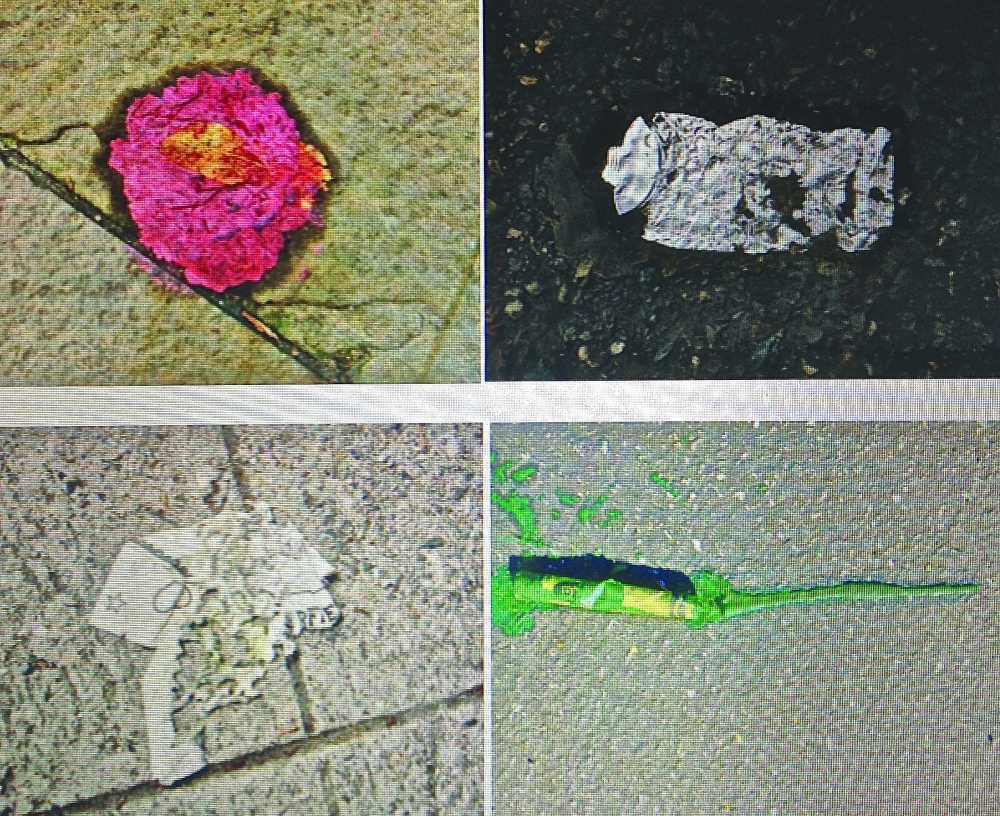
\includegraphics[width=0.8\textwidth]{graphics/FilomenaCruz_RoadKill_ReVista.jpg}
      \caption{Road Kill by Filomena Cruz}
      \label{fig:FilomenaCruz_RoadKill_ReVista}
  \end{figure}

%\item Pictures of Garbage by Vik Muniz
\item \textbf{Pictures of Garbage.} Vic Muniz creates monumental trash art in Jardim Gramacho with the help of \textit{catadores} (Waste Land, 2010) Waste Land, directed by Lucy Walker  tracks the development of a series of monumental photographic portraits made from trash. Called “Pictures of Garbage,” they were created by Mr. Muniz in collaboration with the garbage pickers of Jardim Gramacho, an open-air dump just outside Rio that is one of the largest landfills in Latin America. (Important point is here collaboration with the pickers. Listening their stories and capturing their portraits. What is specific about trash here?)

  \begin{figure}[ht]
      \centering
      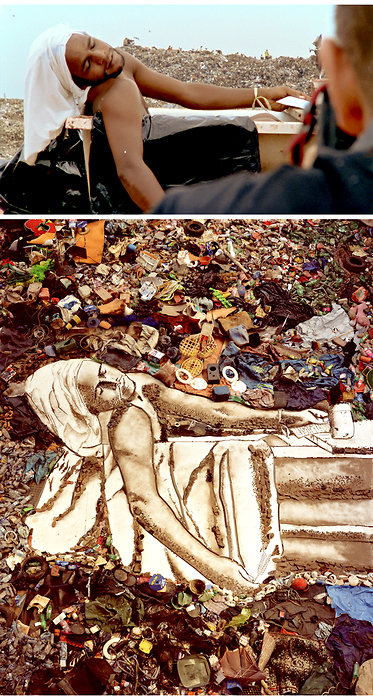
\includegraphics[width=0.5\textwidth]{graphics/vik-muniz-picturesofgarbage0.jpg}
      \caption{Pictures of Garbage by Vic Muniz}
      \label{fig:VicMuniz_PicturesOfGarbage}
  \end{figure}

\item \textbf{The Recycled Orchestra.} Favio Chávez and Nicolás Gómez decide to build musical instruments out of garbage and get 35 children from Cateura, Paraguay’s biggest trash dump, to travel the world with their “Recycled Orchestra”. ``The world send us garbage. We send back music''.

Cateura, Paraguay is a small city that has grown atop a massive dump. It is regarded as one of the poorest slums in Latin America, a village where people live among a sea of garbage. Incredibly, the landfill itself is the primary form of subsistence for many residents, who pick through waste for items that can be used or sold. Prospects for most of the children born in Cateura is bleak as gangs and drugs await many of them. But then one day, something amazing happened. A garbage picker named Nicolás Gómez (known as “Cola”) found a piece of trash that resembled a violin and brought it to musician Favio Chávez. Using other objects collected from the dump, the pair constructed a functional violin in a place where a real violin is worth more a house. Using items gleaned completely from the dump, the pair then built a cello, a flute, a drum, and suddenly had a wild idea: could a children’s orchestra be born in one of the most depressed areas in the world? As you can guess, the answer was yes.

To view scenes from the landfill slum of Cateura in Paraguay is to look into the depths of extreme poverty. But within the contents of the landfill are glimmers of hope in the form of cardboard, utensils and other discarded materials that can be crafted into imperfect but usable musical instruments. These makeshift violins, flutes and cellos, combined with instruction from a local music teacher, have given birth to the Recycled Orchestra of Cateura. Through the music of Mozart, Beethoven and Vivaldi, this orchestra allows the young musicians to transcend their identity as children of poverty.

"A violin is worth more than a house here," says Favio Chavez, the orchestra's director and founder. In the midst of such an existence, these musicians have created something both special and truly awe-inspiring. "My life would be worthless without music." says one girl in pigtails. A young man named Juan Manuel Chavez, nicknamed Bebi, has a cello fashioned out of an oil can and old cooking tools. For the camera, he plays the Prelude to Bach's Cello Suite No. 1 — beautifully.

"People realize that we shouldn't throw away trash carelessly," says Chavez at the end of the trailer. "Well, we shouldn't throw away people either."

This project can be seen as a bricolage practice. They build their musical instruments from what is available around. 

\begin{figure}
    \centering
    \begin{subfigure}[b]{0.3\textwidth}
        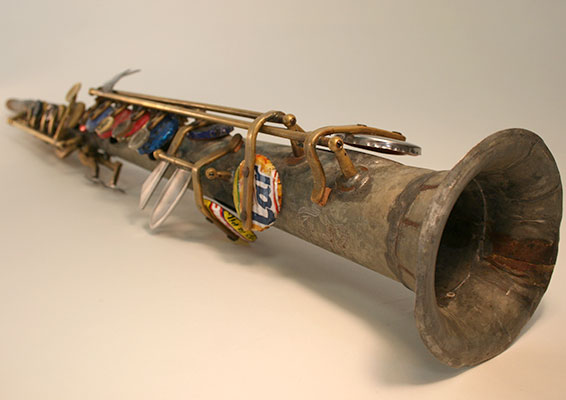
\includegraphics[width=\textwidth]{graphics/landfill_harmonic-sax.jpg}
        \caption{Sax}
        \label{fig:gull}
    \end{subfigure}
    ~ %add desired spacing between images, e. g. ~, \quad, \qquad, \hfill etc. 
      %(or a blank line to force the subfigure onto a new line)
    \begin{subfigure}[b]{0.3\textwidth}
        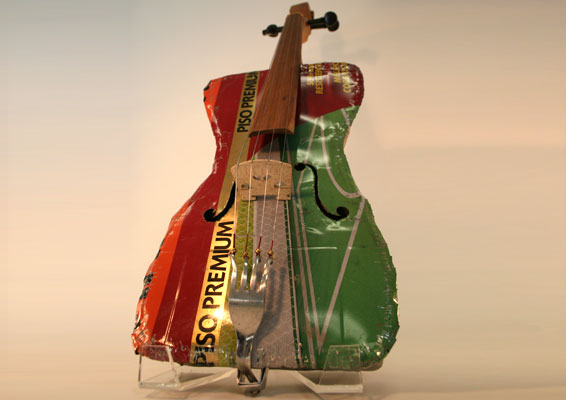
\includegraphics[width=\textwidth]{graphics/landfill_harmonic-violin.jpg}
        \caption{Violin}
        \label{fig:tiger}
    \end{subfigure}
    ~ %add desired spacing between images, e. g. ~, \quad, \qquad, \hfill etc. 
    %(or a blank line to force the subfigure onto a new line)
    \begin{subfigure}[b]{0.3\textwidth}
        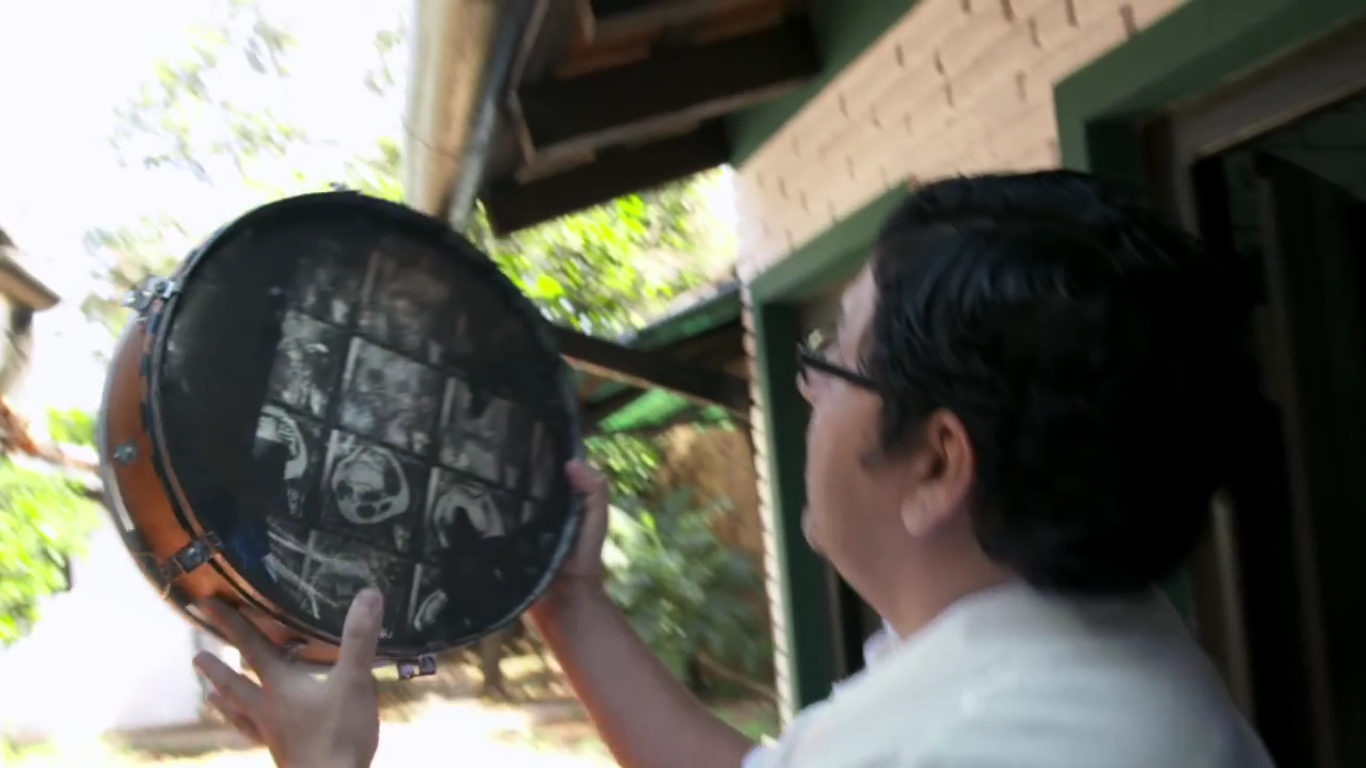
\includegraphics[width=\textwidth]{graphics/landfill_harmonic_drum2.png}
        \caption{Drum}
        \label{fig:mouse}
    \end{subfigure}
    \caption{Instruments of Recycled Orchestra}\label{fig:animals}
\end{figure}

% Beni bu projede etkileyen en öenmli şeyler: ilk olarak oradaki insanların hayatlarını değiştirmesi, hiç hayal edemiyecekleri bir noktaya ulaşmaları, tümünüde kendi emek ve yetenekleriyle başarmaları. yokluk içinden bir şeyler üretmeleri. Her ne kadar üretilen müzik aletleri mükemmel olmasalarda onlar için bulunmayacak bir nimet. Üretilen ürünün kalitesi gerçekten de endüstriyel standartların altında. Müziğin kalitesi diğer kadar olmasa bile farklı bir yaklaşım sunuyor olması önemli. Nasıl oluyor da bu aletten bu ses çıkıyor. Amatör ruhun getirdiği bambaşka bir algı var. Müziğin ötesi, düşündürdüğü bambaşka şeyler var, olaya yeni bir boyut getiriyor. Başka bir alanla diğerinin buluştuğunun bir göstergesi.

% Peki bu iş neden sanat işi olsun ki? 

% Bambaşka şeylere dönüşen ürünler. Üretim amaçlarının dışında. Yeni linkler bağlantılar kuran müzik aletleri. Kendilerinden beklenmeyeni başarmak vs. Daha önce görülmeyen şeyler, görülmeyen ilişkiler.

% http://www.eloisacartonera.com.ar/ENGversion.html
\item “Eloísa Cartonera,” a work cooperative in Buenos Aires, proudly produces handmade books with cardboard covers: \quotes{We purchase [\ldots] cardboard from the
urban pickers (\textit{cartoneros}) who pick it from the streets. Our books are on Latin American literature, the most beautiful we had a chance to read in our lives.} \quotes{Some of them are preserved as art books at university libraries, while others circulate as literary pieces expected to disintegrate in time---something anticipated of the material they are made from.} [from PAOLA IBARRA, ReVista]
  \begin{figure}[ht]
      \centering
      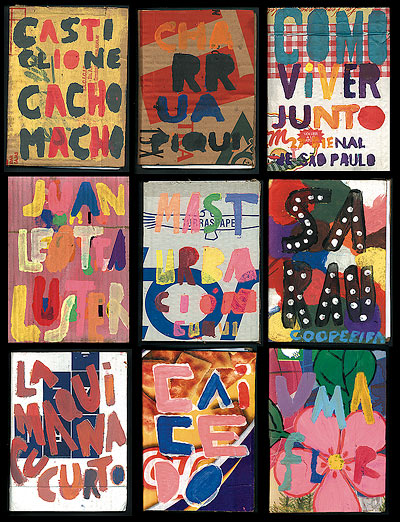
\includegraphics[width=0.5\textwidth]{graphics/EloisaCartonera_Books.jpg}
      \caption{Books covered by Eloisa Cartonera}
      \label{fig:EloisaCartonera_Books}
  \end{figure}

% FROM Paola Ibarra, ReVista
%\item Forever; Blue Yonder by artist Kyle Huffman
%\item Too Too---Much Much by Thomas Hirschhorn
%\item Autoconstrucción by Abraham Cruzvillegas

% FROM Daniel Lind-Ramos BY LOWELL FIET, ReVista
%\item Daniel Lind-Ramos

% FROM A Present from the Sea BY SONIA CABANILLAS, ReVista
% https://www.youtube.com/watch?v=v6IoEF_Tsrw
\item Nick Quijano has some rules to create assemblages. \quotes{There are certain self-imposed rules to this creative process: first, the assemblages or artefactos must all come from material washed ashore on this beach; second, it must be plastic and industrial refuse, result of the processing of fossil fuel; third, it must be polished by a long stay in deep waters, sometimes even encrusted with corals, shells or pebbles, or simply scraped by the ocean floor. As a sign of respect and sacralization, these pieces will be incorporated without any adjustment: no cutting or bending, seen as a mutilation of the object. Its identity cannot be veiled or masked but always must be recognizable amidst the other components; e.g, a comb must remain a comb even as one may see it as a mustache.} The sea returns this refuse; it is not biodegradable.

% FROM Burning Messages BY MICHAEL WELLEN, ReVista
%\item Antonio Berni

% FROM Haiti in the Time of Trash BY LINDA KHACHADURIAN, ReVista
\item Haiti case. When I ask him why he chooses to work in the medium of trash, he replies, \quotes{It gives respect to my city to use the garbage. It shows that everything can be used, and nothing was lost.} (TODO motivation: \quotes{I get more inspiration working with recycled materials because those pieces are unique and can’t be duplicated}) Eugène says that he’s partial to metal, which has become more and more difficult to find because of the clean-up initiative by the city. When I ask him if part of him wishes there were no such effort underway, he answers: \quotes{No. When you have clean streets you have good health, and that is the most important thing.} (This is very strange. It shows that working with trash and being clean healthy is not a contradiction. Both of them exist together.) \quotes{Other people come to Haiti and see junkyards, but we see magical playgrounds,} Jean explains as he watches them.

% FROM Thinking on Film and Trash BY ERNESTO LIVON-GROSMAN, ReVista
% By the 1950s a film like Tire Dié (Fernando Birri, Argentina, 1956) already portrays the collecting, classifying and recycling of trash not only as a source of informal income but as a commercial activity linked to the formal economy. In these films, trash is not the end of a process of consumption but the beginning of a cycle of production. These movies share the idea that trash could be a departure point to think about the modern condition as defined by consumption, class disparities, contamination and urban development. The poet Charles Baudelaire is one of the first to make the connection between the rag picker and the modern city. Walter Benjamin picks it up and from then on the fragmentary condition of trash will remain associated with contemporary art and ultimately with the Modern condition: the industrial refuse could be redeemed by art. It is in this sense that filmmaking becomes allegorical and mimics the process of recycling when it reappropiates archival materials and found footage to create new narratives from scraps, fragments, of films that were not in any way connected to these new narratives.

\item Joseph Cornell

\item \textbf{American Beauty.} The film American Beauty , which features a long, poetic clip of a plastic bag swirling on an eddy of air, snagged five Academy Awards, yet I for one still find it hard to think of plastic bags as things of beauty. 

\item \textbf{Aaron Kramer.} His motto: "Trash is the failure of imagination." \cite{meyer2007turning} In addition to concern for the environment, Kramer was drawn to recycled art because of one simple factor---the price. "Free is certainly great, and that was a driving force for me early on in my career," he said.

\item Nelson’s breakthrough work was The Coral Reef, which he mounted in 2000 at Matt’s Gallery from objects and debris gathered from alleys, trash bins, and car-trunk sales all over London. The title refers to Nelson’s aim of creating an intricate, reeflike network of lives “all existing under one sea, which is capitalism,” he says. (It is very corralate between Ages Varda's work. She shows at the side of human practice, Nelson looks the topic from object side.)

% From http://www.thisiscolossal.com/2014/06/historical-fine-oil-portraits-on-crumpled-trash-by-kim-alsbrooks/, http://www.thisiscolossal.com/2015/05/new-historical-portraits-on-flattened-cans-by-kim-alsbrooks/, http://kimalsbrookswhitetrash.blogspot.com.tr/
\item
\parbox[t]{
	\dimexpr\textwidth-\leftmargin}{%
      \vspace{-2.5mm}
      \begin{wrapfigure}[22]{r}{0.4\textwidth}
        \centering
        \vspace{-\baselineskip}
        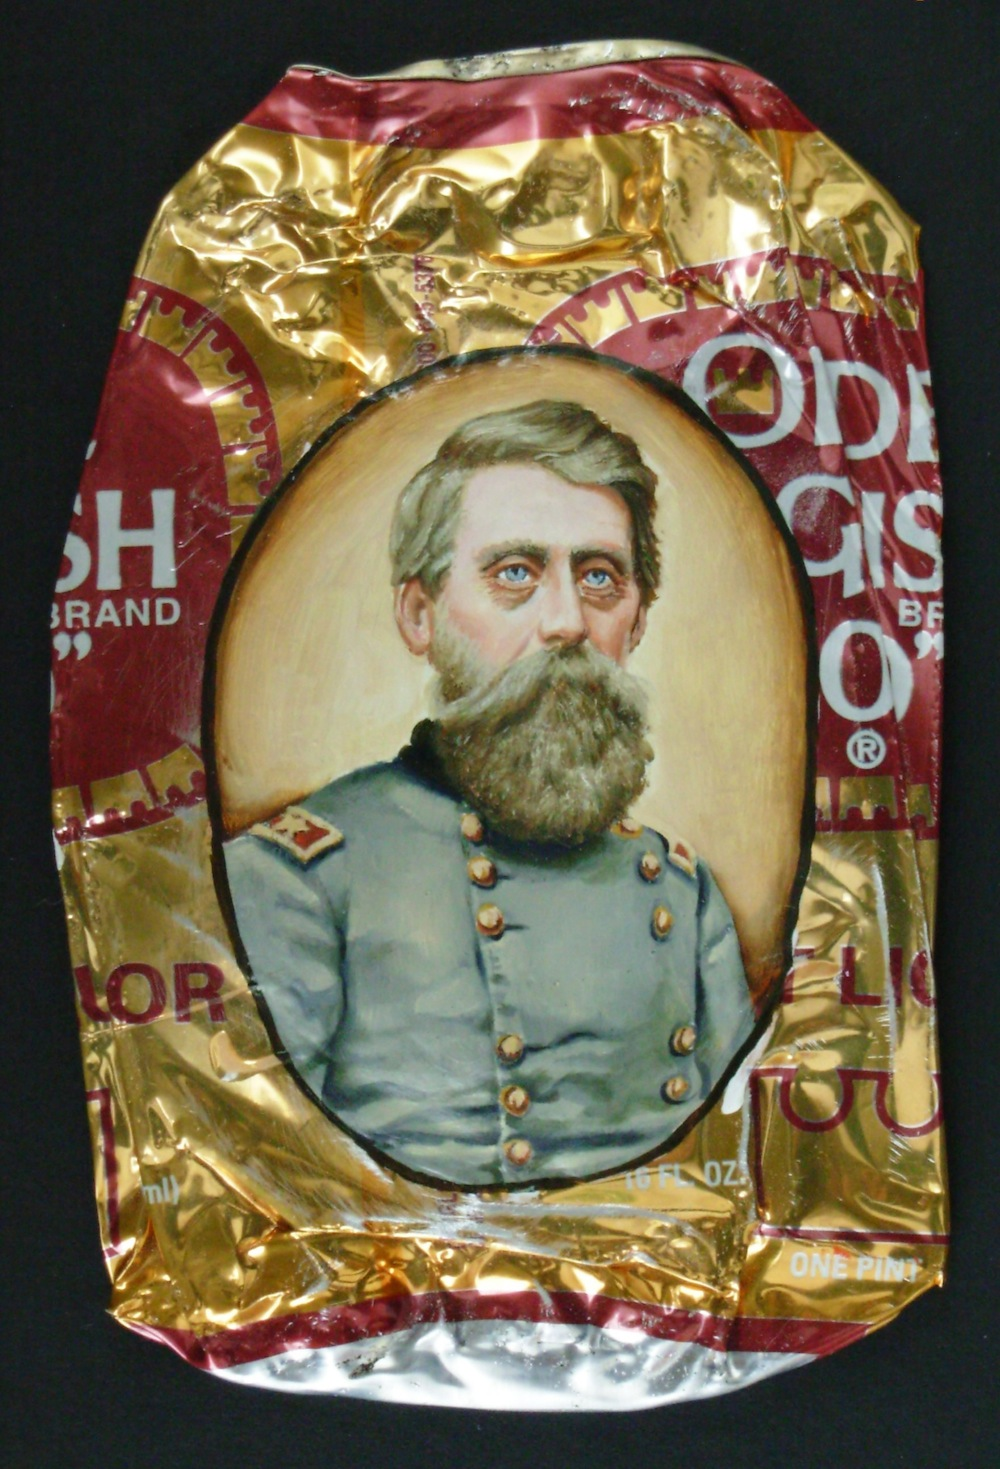
\includegraphics[width=\linewidth]{graphics/Alsbrooks.jpg}
        \caption{The White Trash Series by Kim Alsbrooks}
      \end{wrapfigure}
Kim Alsbrooks, historical oil portraits on flattened beers cans and fast food containers. \quotes{The White Trash Series was developed while living in the South out of frustration with some of the prevailing ideologies, in particular, class distinction. This ideology seems to be based on a combination of myth, biased history and a bizarre sentimentality about old wars and social structures. With the juxtaposition of the portraits from museums, once painted on ivory, now on flattened trash like beer cans and fast food containers, the artist sets out to even the playing field, challenging the perception of the social elite in today’s society.} \quotes{On technique: The trash is found flat, on the street. One cannot flatten the trash. It just doesn't work. It must be found so that there are no wrinkles in the middle and the graphic should be well centered. Then the portraits are found that are complimentary to the particular trash. Generally I depict miniature portraits from the watercolor on ivory era (17th-18th century more or less). The trash is gessoed in the oval shape, image drawn in graphite, painted in oils and varnished.} I need to mention that this images are very subversing to the perception of us about these images. It is unexpected way of presenting images. There is a relationship with the image and painting. At least this work questioned this relation. With tihs work one can ask that with the painting trashed can become valueable thing or with this can this paintiing became valueless. Artsist combines two thing that can be never thought together. New combination, new meaning.}

% Yav biraz da tarihsel fotoğraflara ihtiyaç var mı? aslında bu artworkleri anlatiştaki sıra nasıl olmalı.

\item Martin Kaltwasser \& Folke Föbberling: City As a Resource. One Man's Trash Is Another Man's Treasure. Garbage dump or gold mine? The German artistic collaborators Martin Kaltwasser and Folke Köbberling see rubbish as a major resource. Their projects colonize public space in the name of recycling and design: Overnight, they can make pavilions, villages of huts and even whole houses appear. In installations, exhibitions and, most frequently, guerrilla architectural interventions, they question the conditions of urban life as determined by privatization. For example, in a 2004 project called "Hausbau," they built a house in front of West Berlin's infamous Gropius-designed, failed-utopia high-rise development, Gropiustadt, and moved their family into it for a one week stay; for 2005's "Kleinod," they built a bridge and a stairway between a local family's home and a nearby community garden. In City as a Resource: One Man's Trash Is Another Man's Treasure, Köbberling and Kaltwasser propose simple ways of livening up and re-appropriating the urban habitat with sly alternatives to conventional urban planning. 

Dump or rich source – the "free materials" discovered on the street, on wasteland and on building site rubbish dumps and recycled by Martin Kaltwasser and Folke Köbberling experience incredible metamorphoses. Pavilions, villages of huts and even whole houses are appearing over night. Since 2002 the artists have been using public space as their field of experiment in projects on the use of (free) resources. In installations, exhibitions and most frequently, in actual interventions they question the conditions of urban life determined by privatisation and economisation. Through realised projects the book reveals simple ways of livening up and re-appropriating the City as a Resource and thus offers new components in an alternative to conventional urban planning. Köbberling and Kaltwasser propose informal and self-organised structures rather than the usual methods emphasising control, security and as much marketing as possible. Their approach demonstrates that often – with the help of their own clever building logistics – a huge impact may be made with a minimum of financing.

% From Hold it! : the art & architecture of public-space-bricolage-resistance-resources-aesthetics of Folke Köbberling and Martin Kaltwasser
Public space is under siege. The compulsion to consume, increased monitoring, and continuous traffic expansion will bring fundamental change to the appearance of cities. In 1998, Folke Kobberling and Martin Kaltwasser began implementing their concept of an artistic and architectural aesthetic of resistance to this appropriation. Using 'structural interventions' in streets, squares, bridges, parks and interior spaces they propose alternatives formed of urban 'waste': litter, trash, and other discarded or donated material. 

Köbberling\&Kaltwasser’s large architectural structures attempt to make visible the value of movement and communication through the transformation of found materials into publicly used objects and spaces. Using the city as a field of artistic experimentation, addressing issues of public space and sustainability, their installations, exhibitions and interventions critically question privatisation and economic pressures. The work will be an act of resistance to occupy and reclaim a space and change its meaning. At the same time, the work mirrors the socio-economic aspect of the city - the city as a resource, the materiality of the city, the free material of a city. 

For their projects they use the “city as a resource” and draw on materials they find in urban spaces, for example in containers or on building sites.

Public space and transformed materials. 

% From: http://www.goethe.de/ins/cz/prj/art/kue/koe/enindex.htm
Public space is under siege: pressure to consume, growing control and more and more traffic are threatening to change the picture of our cities dramatically. The couple Folke Köbberling and Martin Kaltwasser have been elaborating their idea of an artistic and architectonical aesthetics of resistance against this take-over since 1998.

They confront consumerist ideologies with alternatives: structural intervention, artistic statements, actions and theories. In doing so, the artists make use of streets, squares, bridges, parks and interiors as operational spaces. And the material they use is always obtained from urban resources: things that have been thrown away, garbage, donated things.

% Sample phrases
% The topic of recycling, presented in this issue, is the "re-use" of materials, objects and structures, for different purposes, and in different ways from their original uses, in order to build or re-build, to provide possible solutions to problems related to the environment, and to manage waste more intelligently. Tyres, containers, bottles, cans, CD-ROMs and even keyboards, can find new and unexpected uses in experimental architecture, exhibition pavilions, or low-cost housing. With recycled objects, one can build anti-seismic and energy efficient houses. Recycled materials can contribute towards building shelters to meet the needs of people affected by disasters. There are many topics connected to recycling, and they vary depending on the objects that one wishes to recycle and how they will be put to use. Used tyres find many applications in REfunc architecture and the Bohlin-Cywinski-Jackson studio. Dorte Mandrup transformed a piezometer into the supporting structure for apartments built with standardized modules. David Hertz reused the wings of a 747 as roof for a villa in Malibu. TYIN Tegnestue architects restored a building with recycled materials, mainly found on location. Yatin Pandya and Footprints E.A.R.T.H. built an activity centre in Ahmedabad using items that were considered as rubbish to their original owners. James & Mau and Infiniski designed fashion homes with recycled containers. The same kind of containers were used by MacArthur Studio and Means & Wells, to build a travelling exhibition pavilion. The GAD. In London, Folke Koebberling and Martin Kaltwasser constructed an experimental theatre using only recycled materials. The panorama that emerges shows the extreme heterogeneity of the work, materials and techniques, the intuitive approach and the infinite possibilities offered by recycling. All of these projects highlight the importance of the construction process as an opportunity for learning and discussion. 

\end{itemize}

Childs can enjoy with trash. I remember from my childhood, we collect crown cap and play with them. Some caps are found less and they worth more. We are looking everywhere for them. To make them flat we put them on the railways. After train passed we get perfect plat cap. At that time it is not trash for us. It has a value and part of our games and enjoy. To have fun a bunch of trash can be enough for us.

In the case of recycling, a dead objects, or an object that reached end of life will begin a new cycle of life. By the artist or other parts are give them a new life. They can reborn as a different things. Do people collect them aware of it? Discarded items unites together with the hands of a artist. 

Trash is global topic men. When you talk about trash, everyone have ideas about it. 

Think a city that has trash monument in the every corner. created from their trash. merged with the city life and gaining unique cityscapes and aesthetics. or think that a museum a trash museum. Exhibits works of art embracing the trash in all aspects. Maybe done by the artist or the visitors from all around world. A place for garbage other than a landfill. Waiting their creator to meet again. What a great idea isn't it? Meeting their creators again. But this time their creator can recognize their trash. They transformed to totally new thing. Reborn. Transformed (Kafka, Gregor Samsa).


%*****************************************
% Maybe...
% Artistic tactics
% Topology of artworks
%*****************************************


%%%
%%%
%%%
\section{Discussions}
Are artworks made from trash just examples of collage and assemblage or more than from them? What about the experience and interaction with other people? Turning art making process to a life practice (or part of life) can be explained in the context of collage (which is mainly related with how a 2d canvas created). But all of them work in fragments, combine many objects together. 

Garbage is often viewed as a form of society’s excess---as the unwanted things that are thrown out without regard. 

In the world of computer science, the term garbage also refers to situations of loss in which data or objects in memory go unused in computer operations.

(Trash has a history. They have different stories. But same destiny?)

Lets make clear the motto: "trash to treasure". What is treasure here. What does it signify? Treasure---something very valuable. from trash. Then it is trash. Not once it is trash. What type of treasure. Who can get value from it. Who creates this treasure? How does it created? Trash is actually is opposite of treasure and then it is switched. In other words trash become treasure and treasure become trash?

Lets consider the practice of working with trash. Why someone believes that discarded objects of people \ldots Looking things that people are refused. Transforming is the one of the most common practice of whole history of man and nature. This practice is forgotten or it is still alive. Agnes Varda actually shows that it is still exist but in different forms. They use it what ruling lifestyle throw out. They are everywhere actually but you should look them carefully. They live in the borders. But live. Event if they are refused they live. Actually it is hard to say that they want to integrate to the system. They want to change it? 

ability of transform, well actually it is very easy to throw away. hard thing is to keep it. force the material. the dimension of trash.

% FROM drink UP, author: Werthan, Sarah, artist: Leech, Gwyneth. A Year in Cups. http://gwynethleech.com/
% trash and art collided. Paper and art, actually paper already medium of art, but is there anything different here. Itself is a part of a work, not the drawing, or painting.
% Documenting via a blog or a website. (what type of dimension it brings the work? maybe connect them, leave message.)
% Buying a beverage is a daily event for \ldots
% Creating art in public places can demystify the process for passers by, Leech says, making artistic expression more accessible and part of people’s everyday lives.
% “People see that an artist can make work anywhere, and make creative spaces anywhere,” she asserts. 

% Trash is as a material or a subject

\begin{itemize}
\item Where do you think this object came from?
\item Why do you think that someone labeled this object as waste?
\item How can you transform this object to tell the story that you thought of before?
\item What story does it tell you?
\item Does it remind you of an event, a specific time in history or in your life, a place, or a state of mind?
\item How can you bring that story to life? (Taylor, 2006, p. 9).
\end{itemize}

% TODO PRAP. from rethink, reimagine, reinvent
Recycling art approach to using reclaimed objects in artworks requires rethinking, or examining the affordances of a particular object to explore the possibilities for the object's inclusion in an artwork. Assemblage art involves the creation of new and innovative objects from what were once considered objects of waste; that is. through their use in assemblage pieces, reclaimed objects are endowed with a new. sometimes paradoxical meaning. The transformations of the objects used in assemblage pieces ask viewers to reconsider the notion of "valuable" as they are challenged to look at everyday objects with a new perspective (Taylor, 2006). Viewers confront issues relating to the functionality of objects during modern processes of production, consumption and distribution.

Artifact exploration promotes historical thinking, literacy investigation, and cultural expression (Higgs \& McNeal, 2006; Levstik \& Barton, 2001; Morris, 1998). Meanings are embedded within cultural artifacts and language (Vygotsky, 1978).

%%
%%
\subsection{What might be the meaning of using trash as a medium in the artworks? Questioning trash as a medium for artist}
\begin{itemize}
\item Some works try to raise awareness the problems that are the result of trash. (It treats environment and nature.)
\item Some of them reflect people's lifestyle especially throw away culture. As a mirror of current lifestyle.
\item Try to find a new value and meaning from the discarded material that are useless anymore. To explore a new approach, new way. Subvert people's ideas about trash and their attitudes by turning materials to the something meaningful (or valuable). Trash to treasure.
\item Using discarded item to represent other discarded things by the ruling ideology or approach. For example, trash can be used to represent refugees. The things that we are trying to discard does not mean that they have no value, instead it means that we have no ability to reveal its potential. In other words, refugees have potential but we see them as players that will change our current system. Therefore, it can be said that willing to transform trash to treasure is to require change of current lifestyle. Rejecting discarding something especially thing that you get value from it is a process and spread through to the ones life.
\item One way is not to produce trash. (Zero trash philosophy.) The other one is to transform trash into something else.
\item What type of experience is that collecting and working on objects that are generally discarded? Experiencing out of common practice, being open to new explorations.
\item Instead of a world that produce trash, how could it be a world created from trash?
\item Combining industrial goods with objects transformed from trash is another way to find a place to trash in the community. It also signifies that trash still has a good quality to used with new materials. Creating composite products from new and reused items. Using the valuable thing with the invaluable thing. It becomes more valuable or less valuable. Depends on the perception.
\item Aesthetics of trash. Revealing aesthetics value of discarded stuff. (Unique visual value. Trash portraits, sculptures etc.)
\end{itemize}


\section{Summary}
Artists works and the place of the trash in the art can be summarized as follow:
\begin{itemize}
\item Artist see them as potential. But what type potential it haves. In which areas. They are already thrown away, if it was value or has a place in the current system they are not thrown away. There is an alternative life and outside of the ruling system.
\item Visual uniqueness, aesthetics dimension.
\end{itemize}

% Ben bölümde aslında çöpün sanatta nasıl yer aldığına bakıyor olacağım. İlk kim kullanmış nasıl kullanmış. Sonrasında hangi anlamlarda kullanılmış. 

% Aslında ben uygun her yerde çöpe olan yaklaşımlarla ilgili örnekler verdim. Peki ya bu bölümde ne yapacağım. Belki gene değineceğim. Ya da ne anlamlara geldiklerini özetleyeceğim. 

% Hangi sonuçlar çıkacak aslında bu bölümden benim için kıymetli olan o. Özellikle caselerden. Bu nasıl bir artistict act oluyor.

% Her sanatçı bu arada çöpü dönüştürmüyor. Bazıları ise onu oldukları gibi kullanıyorlar. Yani farklı kullanım seneryoları var. Ama ben dönüştürmeye dair ne çıkaracağım bu bölümde. 

% aslında dönüştüğünü nereden iddia edebilirim. Rubbish theory? Durable state. Ya da onun tekrar hayata geçtiği. Benimkiler de belli noktalarda fösterilecekler. İnsanlar o defterleri saklıyorlar ne de olsa. Zaten dönüşme işlemi direk müzeye çıkmasıyla oluyor. İllaha onun materyal olarak dönüşmesi gerekmiyor. Bu yüzden her iş aslında bir şekilde dönüştürüyor. Sanatsal pratikler çöpü dönüştürüyorlar. 

% Sanatsal bir eylem olduğuna nasıl varacağım peki? Çünkü topluyorsun, belli bir yaklaşım geliştiriyorsun. Bu eyleme insanları davet ediyorsun. Sanatın eylem olma olayı... Buna burda değinip, kendi işime geçmeliyim.

% Ne topladım buradan. Bu işin sanatsal bağlamdaki yerini öğrendik, yaklaşımları öğrendik. Yeni ihtimaller görme, hayatta var olma, alternatif oluşturma gibi. Ben de bu tür şeyleri kendi işimde kullanacağım.

